\begin{document}
\graphicspath{ {images/naivebayes/} }

\section{Parameter Learning - Naive Bayes Classification}

\subsection{The Naive Bayes Classifier: Introduction}

Previously, we saw how maximum likelihood estimation works for some simple cases. Now, we look at how it works for a more elaborate setup, specifically in the problem of email spam detection. Note that in this section, for simplicity, in showing the maximum likelihood estimates, we will just be setting derivatives equal to 0 without checking second derivatives and boundaries.

We want to build a classifier that, given an email, classifies it as either spam or ham. How do we go about doing the classification? There are many ways to classify data. Today, we're going to talk about one such way called the \textit{naive Bayes classifier}, which uses a simple classification model and has two algorithms to go with it: the first algorithm learns the naive Bayes model parameters from training data, and the second algorithm, given the parameters learned, predicts whether a new email is spam or ham.

Suppose we have $n$ training emails. Email $i$ has a known label $c^{(i)}\in \{ \text {spam},\text {ham}\}$. Also, from email $i$, we extract $J$ features $y^{(i)}=(y_{1}^{(i)},y_{2}^{(i)},\dots ,y_{J}^{(i)})$. In particular, for simplicity, we shall assume that each $y_{j}^{(i)}\in \{ 0,1\}$indicates the presence of the $j$-th word in some dictionary of $J$ words. (Of course, you could use much fancier features such as vector-valued features or even features with non-numerical values, but we'll stick to 0's and 1's that indicate presence of certain words.) For example, maybe the first word in the dictionary is ``viagra'' in which case y1(i) is 1 if email i contains the word ``viagra'' and 0 otherwise. In summary, our training data consists of $y^{(1)},y^{(2)},\dots ,y^{(n)}\in \{ 0,1\} ^{J}$ with respective labels $c^{(1)},c^{(2)},\dots ,c^{(n)}\in \{ \text {spam},\text {ham}\}$.

Next, we specify a probabilistic model that explains how an email is hypothetically generated:

\begin{enumerate}
\item Sample a random label $C$ that is equal to spam with probability $s$ and equal to ham with probability $1-s$. (For example, you could flip a coin with probability of heads $s$, and if the coin comes up heads, you assign $C=spam$, and otherwise you assign $C=ham$.)

\item For $j=1,2, \dots ,J$: Sample $Y_{j}\sim \text {Ber}(q_{j})$ if $C=spam$. Otherwise, sample $Y_{j}\sim \text {Ber}(p_{j})$ if $C=ham$.
\end{enumerate}

Note that the chance of a word from the dictionary occurring depends on whether the email is spam or ham, much like how you'd imagine that if you see the word ``viagra'' in an email, the email's probably spam rather than ham. The above recipe for generating features for a hypothetical email is called a \textit{generative process}, and its corresponding graphical model is as follows:

{\centering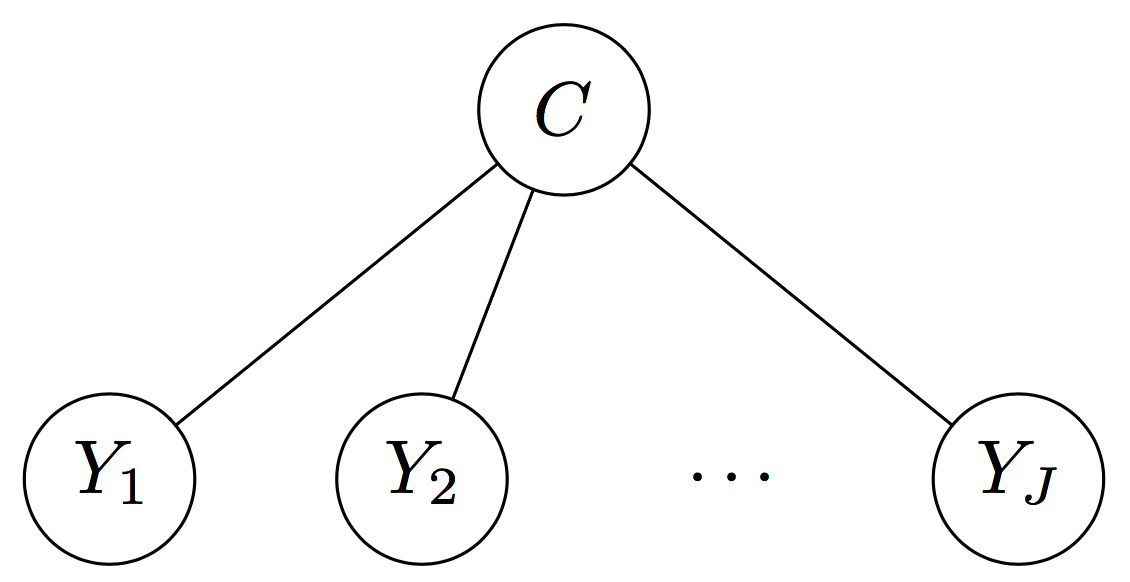
\includegraphics[scale=0.4]{images_naive-bayes} \par}

\textbf{Important observation:} The $Y_i$'s are independent given $C$. This assumption of the model is not actually true for emails since certain words may be more likely to co-occur. Also, the model does not account for the ordering of the words or whether a word occurs multiple times. While the naive Bayes classifier does make these assumptions, in practice, it is often applied to data that violates these assumptions, yet the performance of the classifier is still quite good! To quote statistician George Box, ``All models are wrong but some are useful.''

We need to estimate the parameters $\theta =\{ s,p_{1},p_{2},\dots ,p_{J},q_{1},q_{2},\dots ,q_{J}\}$. We shall assume that our training data $(c^{(i)},y^{(i)})$ for each $i$ are generated i.i.d. according to the above generative process. Then, to learn the parameters, we find $\theta$ that maximizes the likelihood, i.e.:

{\centering$\widehat{\theta } = \arg \max _\theta \prod _{i=1}^ n p_{C, Y_1, \dots , Y_ J}(c^{(i)}, y_1^{(i)}, \dots , y_ J^{(i)}; \theta ).$ \par}


\subsection{The Naive Bayes Classifier: Training}

Note: ``log'' means natural log in these notes.

\textbf{Practice problem:} Show that the log likelihood for our email spam detection setup can be written as

{\centering$\log \left(\prod _{i=1}^{n}p_{C,Y_{1},\dots ,Y_{J}}(c^{(i)},y_{1}^{(i)},\dots ,y_{J}^{(i)};\theta )\right)=f(s)+\sum _{j=1}^{J}g_{j}(p_{j})+\sum _{j=1}^{J}h_{j}(q_{j})$ \par}
 
for some functions $f,g_{1},g_{2},\dots ,g_{J},h_{1},h_{2},\dots ,h_{J}$. What are these functions? Note that what the above equation is saying is that the log likelihood decouples into functions where each function depends on just one of the parameters. Thus, when we want to maximize over $\theta$, what we can do is maximize over each parameter in $\theta$ separately! For example, to find what the ML estimate for $ $s, we only need to look at $(s)$

\textit{Hint:} To show the above equation, you may find it helpful that we can write:

\begin{eqnarray*}
p_C(c; \theta)
&=& s^{\mathbf{1}\{c = \text{spam}\}} (1-s)^{1 - \mathbf{1}\{c = \text{spam}\}}
\qquad\text{for }c\in\{\text{spam}, \text{ham}\} \\
p_{Y_j \mid C}(y_j \mid \text{ham}; \theta)
&=& p_j^{y_j} (1-p_j)^{1 - y_j}
\qquad\text{for }y_j\in\{0, 1\} \\
p_{Y_j \mid C}(y_j \mid \text{spam}; \theta)
&=& q_j^{y_j} (1-q_j)^{1 - y_j}
\qquad\text{for }y_j\in\{0, 1\}
\end{eqnarray*}

\textbf{Practice problem:} After you figure out what the functions $f$, $g_j$'s, and $h_j$'s are, obtain the ML estimate for each of the parameters $s,p_1,\dots ,p_ J,q_1,\dots ,q_ J$ by setting derivatives equal to 0.

\textit{Hint:} You may find it helpful that for nonzero constants $A$ and $B$,

{\centering$\frac{d}{dt}\left\{  A\log t+B\log (1-t)\right\}  =0\qquad \text {when}\qquad t=\frac{A}{A+B}.$ \par} 

\textbf{Simplifying the log likelihood:} The log likelihood is given by

\begin{eqnarray*}
&&\log\left(\prod_{i=1}^{n}p_{C,Y_{1},\dots,Y_{J}}(c^{(i)},y_{1}^{(i)},\dots,y_{J}^{(i)};\theta)\right)\nonumber \\
&&=\log\left(\prod_{i=1}^{n}\left[p_{C}(c^{(i)};\theta)\prod_{j=1}^{J}p_{Y_{j}|C}(y_{j}^{(i)}|c^{(i)};\theta)\right]\right)\nonumber \\
&&=\sum_{i=1}^{n}\left[\log p_{C}(c^{(i)};\theta)+\sum_{j=1}^{J}\log p_{Y_{j}|C}(y_{j}^{(i)}|c^{(i)};\theta)\right]\nonumber \\
&&=\underbrace{\sum_{i=1}^{n}\log p_{C}(c^{(i)};\theta)}_{\text{(*)}}+
\underbrace{\sum_{i=1}^{n}\sum_{j=1}^{J}\log p_{Y_{j}|C}(y_{j}^{(i)}|c^{(i)};\theta)}_{\text{(**)}}.
\end{eqnarray*}

We next simplify the expressions (*) and (**).

First let's simplify term (*):

\begin{eqnarray*}
\text{(*)} &=&\sum_{i=1}^{n}\log p_{C}(c^{(i)};\theta) \\
&=&\sum_{i=1}^{n}\left[\mathbf{1}\{c=``\text{spam}"\}\log s+\mathbf{1}\{c=``\text{ham}"\}\log(1-s)\right]\\
&=&\left[\sum_{i=1}^{n}\mathbf{1}\{c=``\text{spam}"\}\right]\log s+\left[\sum_{i=1}^{n}\mathbf{1}\{c=``\text{ham}"\}\right]\log(1-s)\\
&\triangleq& f(s).
\end{eqnarray*}

Next, we simplify (**), splitting it up as to decouple $p_j$ and $q_j$. To do this, we can split the summation over $i$ into two sums, one accounting for all the ham emails and one accounting for all the spam emails:

\begin{eqnarray*}
&&\text{(**)} \\
&&=\sum_{i=1}^{n}\sum_{j=1}^{J}\log p_{Y_{j}|C}(y_{j}^{(i)}|c^{(i)};\theta)\\
&&=\sum_{i=1}^{n}\mathbf{1}\{c^{(i)}=``\text{ham}"\}\sum_{j=1}^{J}\log p_{Y_{j}|C}(y_{j}^{(i)}|c^{(i)};\theta)\\
&&\quad+\sum_{i=1}^{n}\mathbf{1}\{c^{(i)}=``\text{spam}"\}\sum_{j=1}^{J}\log p_{Y_{j}|C}(y_{j}^{(i)}|c^{(i)};\theta)\\
&&=\sum_{i=1}^{n}\mathbf{1}\{c^{(i)}=``\text{ham}"\}\sum_{j=1}^{J}\left[y_{j}^{(i)}\log p_{j}+(1-y_{j}^{(i)})\log(1-p_{j})\right]\\
&&\quad+\sum_{i=1}^{n}\mathbf{1}\{c^{(i)}=``\text{spam}"\}\sum_{j=1}^{J}\left[y_{j}^{(i)}\log q_{j}+(1-y_{j}^{(i)})\log(1-q_{j})\right] \\
&&=\sum_{j=1}^{J}\underbrace{\sum_{i=1}^{n}\mathbf{1}\{c^{(i)}=``\text{ham}"\}\left[y_{j}^{(i)}\log p_{j}+(1-y_{j}^{(i)})\log(1-p_{j})\right]}_{\triangleq g_{j}(p_{j})}\\
&&\quad+\sum_{j=1}^{J}\underbrace{\sum_{i=1}^{n}\mathbf{1}\{c^{(i)}=``\text{spam}"\}\left[y_{j}^{(i)}\log q_{j}+(1-y_{j}^{(i)})\log(1-q_{j})\right]}_{\triangleq h_{j}(q_{j})}.
\end{eqnarray*}

In summary:

\begin{eqnarray*}
f(s) &=&\left[\sum_{i=1}^{n}\mathbf{1}\{c^{(i)}=``\text{spam}"\}\right]\log s+\left[\sum_{i=1}^{n}\mathbf{1}\{c^{(i)}=``\text{ham}"\}\right]\log(1-s),\\
g_{j}(p_{j}) &=&\left[\sum_{i=1}^{n}\mathbf{1}\{c^{(i)}=``\text{ham}"\}y_{j}^{(i)}\right]\log p_{j}+\left[\sum_{i=1}^{n}\mathbf{1}\{c^{(i)}=``\text{ham}"\}(1-y_{j}^{(i)})\right]\log(1-p_{j}),\\
h_{j}(q_{j}) &=&\left[\sum_{i=1}^{n}\mathbf{1}\{c^{(i)}=``\text{spam}"\}y_{j}^{(i)}\right]\log q_{j}+\left[\sum_{i=1}^{n}\mathbf{1}\{c^{(i)}=``\text{spam}"\}(1-y_{j}^{(i)})\right]\log(1-q_{j}).
\end{eqnarray*}

\textbf{Setting derivatives to 0:} The ML estimate for $s$ is $\widehat{s}=\arg \max _{s\in [0,1]}f(s)$, which occurs when $\frac{df}{ds}=0$. Using the hint, we see that

{\centering$f(s)=\underbrace{\left[\sum _{i=1}^{n}\mathbf{1}\{ c^{(i)}=``\text {spam}"\} \right]}_{A}\log s+\underbrace{\left[\sum _{i=1}^{n}\mathbf{1}\{ c^{(i)}=``\text {ham}"\} \right]}_{B}\log (1-s)$ \par}
 
has derivative equal to 0 when

{\centering$\widehat{s}=\frac{A}{A+B}=\frac{\sum _{i=1}^{n}\mathbf{1}\{ c^{(i)}=``\text {spam}"\} }{\sum _{i=1}^{n}\mathbf{1}\{ c^{(i)}=``\text {spam}"\} +\sum _{i=1}^{n}\mathbf{1}\{ c^{(i)}=``\text {ham}"\} }=\frac{\sum _{i=1}^{n}\mathbf{1}\{ c^{(i)}=``\text {spam}"\} }{n}.$ \par}
 
This result is intuitive -- it's the number of emails labeled ``spam'' divided by the total number of emails.

The ML estimate for $p_j$ is $\widehat{p}_{j}=\arg \max _{p_{j}\in [0,1]}g_{j}(p_{j})$, which occurs when $\frac{dg_{j}}{dp_{j}}=0$. Again using the hint, we see that

{\centering$g_{j}(p_{j})=\underbrace{\left[\sum _{i=1}^{n}\mathbf{1}\{ c^{(i)}=``\text {ham}"\} y_{j}^{(i)}\right]}_{A}\log p_{j}+\underbrace{\left[\sum _{i=1}^{n}\mathbf{1}\{ c^{(i)}=``\text {ham}"\} (1-y_{j}^{(i)})\right]}_{B}\log (1-p_{j})$ \par}
 
has derivative equal to 0 when

\begin{eqnarray*}
\widehat{p}_{j} & =&\frac{A}{A+B}\\
 & =&\frac{\sum_{i=1}^{n}\mathbf{1}\{c^{(i)}=``\text{ham}"\}y_{j}^{(i)}}{\sum_{i=1}^{n}\mathbf{1}\{c^{(i)}=``\text{ham}"\}y_{j}^{(i)}+\sum_{i=1}^{n}\mathbf{1}\{c^{(i)}=``\text{ham}"\}(1-y_{j}^{(i)})}\\
 & =&\frac{\sum_{i=1}^{n}\mathbf{1}\{c^{(i)}=``\text{ham}"\}y_{j}^{(i)}}{\sum_{i=1}^{n}\mathbf{1}\{c^{(i)}=``\text{ham}"\}}.
\end{eqnarray*}

This result is also intuitive -- it's the number of times word $j$ occurred in an email labeled ``ham'' divided by the total number of emails labeled ``ham''.

Finally, by pattern-matching, the ML estimate for $q_j$ is

{\centering$\widehat{q}_{j}=\frac{\sum _{i=1}^{n}\mathbf{1}\{ c^{(i)}=``\text {spam}"\} y_{j}^{(i)}}{\sum _{i=1}^{n}\mathbf{1}\{ c^{(i)}=``\text {spam}"\} }.$ \par}
 
Wonderful, now we can write up an algorithm that computes all those ML estimates above. Once we learn the parameters $\theta$, we can treat them as fixed and start doing prediction.


\subsection{The Naive Bayes Classifier: Prediction}

\textbf{Practice problem:} Once we learn the parameters $\theta$, we can treat them as fixed and start doing prediction. Let's now look at classifying whether a new email that's not in our training data is spam or ham. This new email has random, unobserved label $C$, which we would like to infer, but we only get to see its features $Y_{1} = y_1,Y_{2} = y_2,\dots ,Y_{J} = y_ J$. Assuming that $\theta$ is known and fixed, figure out what the MAP estimate for label $C$ is given $Y_{1} = y_1,Y_{2} = y_2,\dots ,Y_{J} = y_ J$.

Unleashing Bayes' rule,

\begin{eqnarray*}
 &&p_{C|Y_{1},\dots,Y_{J}}(``\text{spam}"|y_{1},\dots,y_{J})\\
 &&=\frac{p_{C}(``\text{spam}")p_{Y_{1},\dots,Y_{J}|C}(y_{1},\dots,y_{J}|``\text{spam}")}{p_{Y_{1},\dots,Y_{J}}(y_{1},\dots,y_{J})}\\
 &&=\frac{p_{C}(``\text{spam}")p_{Y_{1},\dots,Y_{J}|C}(y_{1},\dots,y_{J}|``\text{spam}")}{p_{C}(``\text{spam}")p_{Y_{1},\dots,Y_{J}|C}(y_{1},\dots,y_{J}|``\text{spam}")+p_{C}(``\text{ham}")p_{Y_{1},\dots,Y_{J}|C}(y_{1},\dots,y_{J}|``\text{ham}")} \\
 &&=\frac{p_{C}(``\text{spam}")\prod_{j=1}^{J}p_{Y_{j}|X}(y_{j}|``\text{spam}")}{p_{C}(``\text{spam}")\prod_{j=1}^{J}p_{Y_{j}|C}(y_{j}|``\text{spam}")+p_{C}(``\text{ham}")\prod_{j=1}^{J}p_{Y_{j}|X}(y_{j}|``\text{ham}")}\\
 &&=\frac{s\prod_{j=1}^{J}q_{j}^{y_{j}}(1-q_{j})^{1-y_{j}}}{s\prod_{j=1}^{J}q_{j}^{y_{j}}(1-q_{j})^{1-y_{j}}+(1-s)\prod_{j=1}^{J}p_{j}^{y_{j}}(1-p_{j})^{1-y_{j}}},
\end{eqnarray*}

where for simplicity we've dropped the hats on the parameters even though the parameter values we use are estimated from training data.

Of course,

\begin{eqnarray*}
&&p_{C|Y_{1},\dots,Y_{J}}(``\text{ham}"|y_{1},\dots,y_{J}) \\
&&= 1 - p_{C|Y_{1},\dots,Y_{J}}(``\text{spam}"|y_{1},\dots,y_{J}) \\
&&=
\frac{(1-s)\prod_{j=1}^{J}p_{j}^{y_{j}}(1-p_{j})^{1-y_{j}}}{s\prod_{j=1}^{J}q_{j}^{y_{j}}(1-q_{j})^{1-y_{j}}+(1-s)\prod_{j=1}^{J}p_{j}^{y_{j}}(1-p_{j})^{1-y_{j}}}.
\end{eqnarray*}

The MAP estimate for $C$ is

\begin{eqnarray*}
\widehat{C}_{\text{MAP}}
&=&
\begin{cases}
``\text{spam}"
& \text{if }
p_{C|Y_{1},\dots,Y_{J}}(``\text{spam}"|y_{1},\dots,y_{J})
\ge p_{C|Y_{1},\dots,Y_{J}}(``\text{ham}"|y_{1},\dots,y_{J}) \\
``\text{ham}"
& \text{otherwise}.
\end{cases}
\end{eqnarray*}

Note that here we're breaking ties in favor of spam. The above is equivalent to looking at whether the odds ratio

{\centering$\frac{p_{C|Y_{1},\dots ,Y_{J}}(``\text {spam}"|y_{1},\dots ,y_{J})}{p_{C|Y_{1},\dots ,Y_{J}}(``\text {ham}"|y_{1},\dots ,y_{J})}$ \par}
 
is at least 1, or whether the log odds ratio

{\centering$\log \frac{p_{C|Y_{1},\dots ,Y_{J}}(``\text {spam}"|y_{1},\dots ,y_{J})}{p_{C|Y_{1},\dots ,Y_{J}}(``\text {ham}"|y_{1},\dots ,y_{J})}$ \par}

is at least 0. In practice the log odds ratio can be much more numerically stable to compute since, pushing in the log, we end up taking sums and differences of log probabilities rather than multiplying a large number of probabilities.

\subsection{The Naive Bayes Classifier: Laplace Smoothing}

\textbf{Practice problem:} Assume that a particular word, say word 1, did not appear in any of the training data. Now for the email we're trying to predict the label for, suppose that we observe that $y_1=1$. What is $p_{Y_{1},\dots ,Y_{J}}(y_{1},\dots ,y_{J})$? What went wrong? Can you think of a way to modify the prediction step to address this issue?

Assume that a particular word, say word 1, did not appear in any of the training data. Now for the email we're trying to predict the label for, suppose that we observe that $y_1=1$. We would have learned that $p_{1}=q_{1}=0$ (we're leaving hats off to keep notation from getting cluttered). Using the result of the prediction phase, we see that

{\centering$p_{Y_{1},\dots ,Y_{J}}(y_{1},\dots ,y_{J})=s\prod _{j=1}^{J}q_{j}^{y_{j}}(1-q_{j})^{1-y_{j}}+(1-s)\prod _{j=1}^{J}p_{j}^{y_{j}}(1-p_{j})^{1-y_{j}}=0$ \par}
 
since $y_1=1$ while $p_{1}=q_{1}=0$. In other words, the observation is impossible given the model learned! Hence, computing $\mathbb {P}(C=\text {spam}|Y_{1}=1,Y_{2}=y_{2},\dots ,Y_{J}=y_{J})$ doesn't make sense since we're conditioning on an event that has 0 probability.

Thus, ML estimates aren't robust in this case to words that we don't encounter in training data.

One way to resolve this is to take a Bayesian approach to parameter estimation (we saw this earlier when we put a prior on the bias of a coin) and, in particular, introduce pseudocounts. For example, we could set:

\begin{eqnarray*}
\widehat{s} & =&\frac{\sum_{i=1}^{n}\mathbf{1}\{c^{(i)}=``\text{spam}"\}+1}{n+2},\\
\widehat{p}_{j} & =&\frac{\sum_{i=1}^{n}\mathbf{1}\{c^{(i)}=``\text{ham}"\}y_{j}^{(i)}+1}{\sum_{i=1}^{n}\mathbf{1}\{c^{(i)}=``\text{ham}"\}+2},\\
\widehat{q}_{j} & =&\frac{\sum_{i=1}^{n}\mathbf{1}\{c^{(i)}=``\text{spam}"\}y_{j}^{(i)}+1}{\sum_{i=1}^{n}\mathbf{1}\{c^{(i)}=``\text{spam}"\}+2}.
\end{eqnarray*}
 
This ensures that none of the parameters are estimated as 0 or 1.

Note that introducing a pseudocount for each possible outcome has a special name: Laplace smoothing, also called additive smoothing. For $\widehat{s}$, this means introducing 1 pseudocount for spam and 1 pseudocount for ham. For $\widehat{p}_{j}$, this means introducing 1 pseudocount for word $j$ appearing in ham and 1 pseudocount for word $j$ not appearing in ham. You could, of course, also introduce $\ell$ pseudocounts for each possible outcome instead of just one, i.e.,

\begin{eqnarray*}
\widehat{s} & =&\frac{\sum_{i=1}^{n}\mathbf{1}\{c^{(i)}=``\text{spam}"\}+\ell}{n+2\ell},\\
\widehat{p}_{j} & =&\frac{\sum_{i=1}^{n}\mathbf{1}\{c^{(i)}=``\text{ham}"\}y_{j}^{(i)}+\ell}{\sum_{i=1}^{n}\mathbf{1}\{c^{(i)}=``\text{ham}"\}+2\ell},\\
\widehat{q}_{j} & =&\frac{\sum_{i=1}^{n}\mathbf{1}\{c^{(i)}=``\text{spam}"\}y_{j}^{(i)}+\ell}{\sum_{i=1}^{n}\mathbf{1}\{c^{(i)}=``\text{spam}"\}+2\ell}.
\end{eqnarray*}

\end{document}
